\section{Белые карлики: основные свойства, образование, новые и сверхновые типа Ia}
\subsection{Общие сведения}
Белые карлики -- компактные объекты большой плотности, образующиеся в результате эволюции звёзд не привыкающих массы $\sim 10M_{\Sun}$. Когда звезда главной последовательности малой или средней массы заканчивает превращение водорода в гелий, она расширяется, становясь красным гигантом. Красный гигант поддерживается термоядерными реакциями превращения гелия в углерод и кислород. Если масса красного гиганта оказывается недостаточной для подъёма температуры ядра до уровня, необходимого для термоядерных реакций с участием полученного углерода, происходит его накопление в ядре звезды, вместе с кислородом. Звезда сбрасывает внешнюю оболочку, формируя планетарную туманность, а бывшее ядро звезды становится белым карликом, состоящим из углерода и кислорода.

Ближайший известный белый карлик — Сириус B, находящийся на расстоянии в 8,6 световых лет. В настоящее время белые карлики составляют, по разным оценкам, от 3 до 10\% звёздного населения нашей галактики (неопределённость оценки обусловлена трудностью наблюдения удалённых белых карликов из-за их малой светимости).

В зависимости от исходной массы звезды, термоядерные реакции также могут остановиться на гелии (для звёзд с очень малой массой, характерных для двойных звёздных систем) или на неоне (для звёзд массой от 8 до 10,5 солнечных), что приведёт к образованию белых карликов, состоящих соответственно из гелия или кислорода, неона и магния.

Образующийся объект имеет массу порядка солнечной, однако его диаметр может быть в $\sim 100$ раз меньше.  
\subsection{Предел Чандрасекара}
Как уже упоминалось, массы белых карликов составляют порядка солнечной, но размеры составляют лишь сотую (и даже меньше) часть солнечного радиуса, то есть плотность вещества в белых карликах чрезвычайно высока и составляет $\rho \sim 10^{5}-10^{9} \ \frac{\text{г}}{\text{см}^{3}} $. При таких плотностях электронные оболочки атомов разрушаются, и вещество представляет собой электронно-ядерную плазму, причём её электронная составляющая представляет собой вырожденный электронный газ. Давление $P$ такого газа подчиняется следующей зависимости:
\begin{equation*}
    P = K\rho^{\frac{5}{3}}
\end{equation*}
Вышеприведённое уравнение состояния действительно для холодного электронного газа, но температура даже в несколько миллионов градусов мала по сравнению с характерной ферми-энергией электронов (
$kT\ll E_{F}$). Вместе с тем, при росте плотности вещества из-за запрета Паули (два электрона не могут иметь одно квантовое состояние, то есть одинаковую энергию и спин), энергия и скорость электронов возрастают настолько, что начинают действовать эффекты теории относительности — вырожденный электронный газ становится релятивистским. Зависимость давления $P$ релятивистского вырожденного электронного газа от плотности уже другая:
\begin{equation*}
    P = K\rho^{\frac{4}{3}}
\end{equation*}
Средняя плотность белого карлика ($M$ -- его масса, $R$ -- радиус):
\begin{gather*}
    \rho \propto \frac{M}{R^{3}}\\
    P\propto \frac{M^{\frac{4}{3}}}{R^{4}}
\end{gather*}
Cила давления, противодействующая гравитации и равная перепаду давления по глубине:
\begin{equation*}
    \frac{P}{R}\propto \frac{M^{\frac{4}{3}}}{R^{5}}
\end{equation*}
Гравитационные силы, противодействующие давлению:
\begin{equation*}
    \frac{\rho G M}{R^{2}} \propto \frac{M^{2}}{R^{5}}
\end{equation*}
то есть, хотя перепад давления и гравитационные силы одинаково зависят от радиуса, но по-разному зависят от массы. Следствием такого соотношения зависимостей является существование некоторого значения массы звезды, при которой гравитационные силы уравновешиваются силами давления, а при увеличении массы белого карлика его радиус уменьшается. Другим следствием является то, что если масса больше некоторого предела (предел Чандрасекара), то звезда коллапсирует. Предел Чандрасекара -- $1.2M_{\Sun}$. 
\begin{figure}[H]
    \centering
    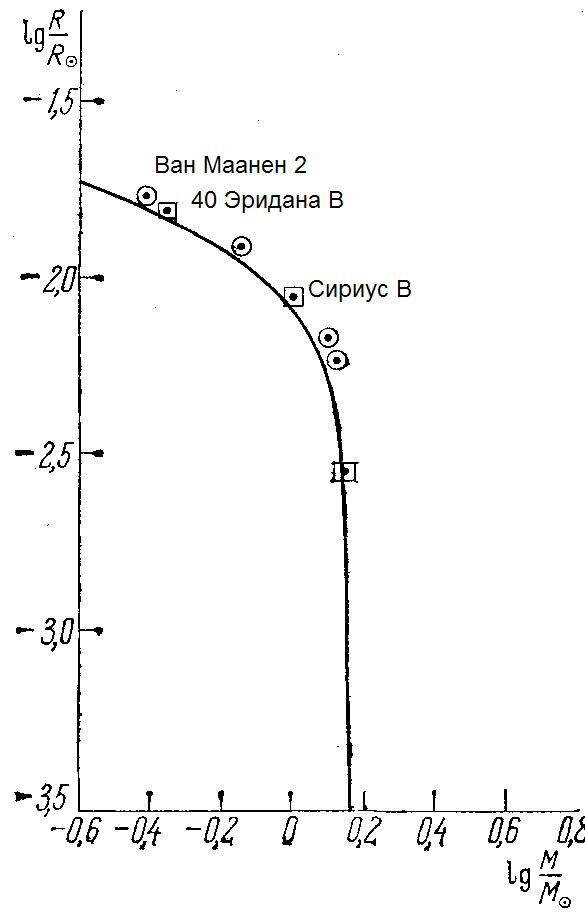
\includegraphics[scale=0.5]{white_dwarf.png}
    \caption{Кривая радиус -- масса (нормированная и логарифмированная) для белых карликов.}
    \label{fig:wd}
\end{figure}
\subsection{Сверхновые типа Ia}
\subsection{Аккреционный механизм}
Если белый карлик является одной из звёзд двойной системы, то он может начать аккрецировать массу со второй звезды, тем самым наращивая свою массу. В некоторых случаях накопив массу близкую к пределу Чандрасекара карлик может взорваться сверхновой.

При взрыве температура в ядре достигает миллиарда градусов, а значительная часть вещества белого карлика, состоявшего в основном из кислорода и углерода, за несколько секунд превращается в более тяжёлые элементы и выбрасывается в окружающее пространство со скоростями до 5 000 — 20 000 км/с, что составляет примерно 6 \% от скорости света. Выделенной энергии ($1—2\cdot10^{44}$ Дж) достаточно чтобы полностью разорвать звезду, то есть отдельные её составляющие части получают достаточно кинетической энергии, чтобы преодолеть гравитацию.
\subsection{Механизм слияния}
Существует и другой механизм запуска термоядерных реакций. Белый карлик может слиться с другим белым карликом (не менее 80\% всех сверхновых Ia типа по одним данным, менее 15 \% или даже как чрезвычайно редкое по другим) и на короткое время может превысить предел массы и начать коллапсировать, снова поднимая свою температуру до достаточной для ядерного синтеза. В течение нескольких секунд после начала ядерного синтеза со значительной частью вещества белого карлика происходит быстрая термоядерная реакция с выделением большого количества энергии ($1—2\cdot10^{44}$ Дж), вызывающая взрыв сверхновой звезды.
